%Preamble
\pdfminorversion=4
\documentclass[12pt]{article}
\usepackage[spanish]{babel}
\usepackage[utf8x]{inputenc}
\usepackage{tabularx} % extra features for tabular environment
\usepackage{amsmath}  % improve math presentation
\usepackage{graphicx} % takes care of graphic including machinery
\usepackage{geometry} % decreases margins
\usepackage{cite} % takes care of citations
\usepackage[final]{hyperref} % adds hyper links inside the generated pdf file
\usepackage{booktabs}
\usepackage{subcaption}
\usepackage{fancyhdr}
\usepackage{parskip}
\usepackage{amssymb, amsmath} % Paquetes matemáticos de la American Mathematical Society
\usepackage{float}
%\usepackage{showframe}

\geometry{
    papersize = {216mm, 279mm},
    width = 16.6cm,
    height = 25cm,
    headsep = 5mm,
    head = 2.8cm,
    marginpar = 5mm,
    includeall,
}

\fancyhf{}
\renewcommand{\headrulewidth}{0pt}
\fancyhead[LO,LE]{
    \begin{minipage}{3cm}
        
\includegraphics[width=0.7\textwidth]{Escudo.jpg}
    \end{minipage}
}
\fancyhead[RO,RE]{
    \textsf{
        Serie de Fourier aplicado a una función Diente de Sierra\\
        Teoría de telecomunicaciones I, Grupo A12\\
        \date{\today}.   
    }
}
\fancyfoot[C]{\thepage}

\pagestyle{fancy}

\hypersetup{
	colorlinks=true,       % false: boxed links; true: colored links
	linkcolor=black,        % color of internal links
	citecolor=black,        % color of links to bibliography
	filecolor=magenta,     % color of file links
	urlcolor=blue         
}
\spanishdecimal{.}

%++++++++++++++++++++++++++++++++++++++++
%Content

\title{\textbf{Series de Fourier}}
\author{
    Jefry Nicolás Chicaiza - \url{jefryn@unicauca.edu.co}\\
    Jose Nicolás Zambrano - \url{jnzambranob@unicauca.edu.co}
}
\date{}

\begin{document}
\maketitle
\thispagestyle{fancy}
\section*{Introducción}
    En el siguiente documento se desarrollará el informe del Trabajo 1 de la asignatura 
    Teoría de las telecomunicaciones 1. El trabajo presenta inicialmente el desarrollo 
    analítico mediante serie de Fourier de la señal planteada, la cual es del tipo 
    "diente de sierra"  trasladado en el tiempo.\\
    \\
    Iniciar con el desarrollo analítico es necesario debido a que para alcanzar los 
    resultados esperados en la simulación, se requiere conocer de antemano los coeficientes 
    de la serie de Fourier que permitirán reconstruir la señal a través de iteraciones 
    realizadas con MATLAB.\\
    \\
    Posteriormente se abordaran las hipótesis planteadas en el documento guiá del trabajo 
    y se buscará llegar a conclusiones y síntesis a partir de los datos obtenidos en la 
    simulación de los diferentes escenarios.\\
    \\
    Los teoremas e hipótesis nos dicen que la serie de Fourier de cualquier señal periódica de potencia 
    finita la podemos obtener por medio de una suma infinita de funciones sinusoidales. La serie de 
    Fourier de una señal pueden expresarse de dos maneras, una representada por serie trigonométrica y 
    otra con representación de serie compleja.\\ 
    \\
    En este documento unicamente se realiza los cálculos de la serie de Fourier para la señal propuesta 
    con la representación trigonométrica, que observamos a continuación:

    \begin{equation}
        x(t)=a_{0}+\sum_{n=1}^{\infty} a_{n}cos(2\pi nf_{0}t)+b_{n}sin(2\pi f_{0}t)
        \label{equation1}
    \end{equation}
    
    Donde los términos $a_{0}$, $a_{n}$ y $b_{n}$ son los coeficientes de la serie de Fourier, de los cuales
    es necesario realizar cálculos para encontrar sus valores y lograr representar la serie de la señal dada.\\
    \\
    El desarrollo de este documento esta constituido por una sesión que brinda información 
    de como se obtuvo las diferentes expresiones y el plan de pruebas, que hacen posible la 
    realización de diferentes escenarios para la simulación. \\
    \\

    

    Recuerden que cantidad no necesariamente implica calidad, por lo que la mejor apuesta 
    es ser concisos y no crear un Frankenstein com información de otras fuentes, dicho de 
    otra forma "no pasen a sucio lo que ya está en limpio".\\
    \\
    Una vez aclarado el punto anterior, en mi opinión la introducción se debe utilizar 
    principalmente para dos cosas:
    \begin{enumerate}
        \item Contextualizar. En esta parte deben indicar por qué y el para qué se su informe 
        (no vale decir que es para pasar el curso), pueden introducir definiciones 
        importantes o conceptos teóricos necesarios para entender el resto del 
        documento. No obstante, no se trata de elaborar un marco teórico.

        \item Enunciar. Dado que ya se ha explicado la finalidad de su trabajo, se debe mostrar 
        de forma concisa la forma en la que éste se ha desarrollado, como un abrebocas 
        para que el lector sepa qué es lo que encontrará más adelante. Esta segunda 
        parte es mejor escribirla una vez haya terminado el resto del documento.
    \end{enumerate}
    Deben tener presente que en muchos casos de la introducción depende que una persona 
    continúe leyendo (yo soy la estoica excepción), por lo que traten de que quede muy clara la 
    primera parte de la introducción, para lo cual deben seguir un hilo conductor y una 
    secuencia lógica. En mi caso es muy útil definir primero qué quiero decir en cada párrafo 
    antes de comenzar a escribirlo.\\
    \\
    Aunque cada persona tiene su propio estilo de escritura, para mi es una buena táctica 
    plantear preguntas dentro del texto que nos ayuden a conducir al lector por el tema, una 
    pregunta bien planteada puede ser muy valiosa por sí sola.\\
    \\
    En cuanto a la redacción deben tener una cosa muy clara, NO DEBEN ESCRIBIR EN 
    PRIMERA PERSONA y deben intentar ser claros con respecto a sus afirmaciones.
    
\section*{Metodología}
    La metodología empleada para el desarrollo de la serie de Fourier a la señal planteada se 
    logro mediante la aplicación de los teoremas e hipótesis, en el apartado anterior se menciono 
    la necesidad de calcular los valores de ciertos términos para logra obtener la representación 
    matemática de la serie de Fourier de la señal planteada.\\ 
    \\
    En primer lugar es importante conocer el comportamiento que nos describe los términos, el primer 
    termino de la serie, $a_{0}$, no está asociado con una frecuencia y es una constante, además es 
    conocido como el nivel DC de la señal, representa el cambio de la señal sobre un nivel arbitrario 
    de referencia. Este termino lo podemos calcular de la siguiente manera:

    \begin{equation}
        a_{0}=\frac{1}{T} \int_{T}^{} x(t)dt
        \label{equation2}
    \end{equation}
    
    De la expresión anterior podemos deducir que el termino DC representa el área bajo la curva de la 
    señal \cite{diapositivas}, que hasta el momento no conocemos la función que la representa, por tanto es necesario obtener 
    la función a partir de su gráfica. En la figura \ref{figure1} observamos la señal asignada.

    \begin{figure}[H]
        \centering
        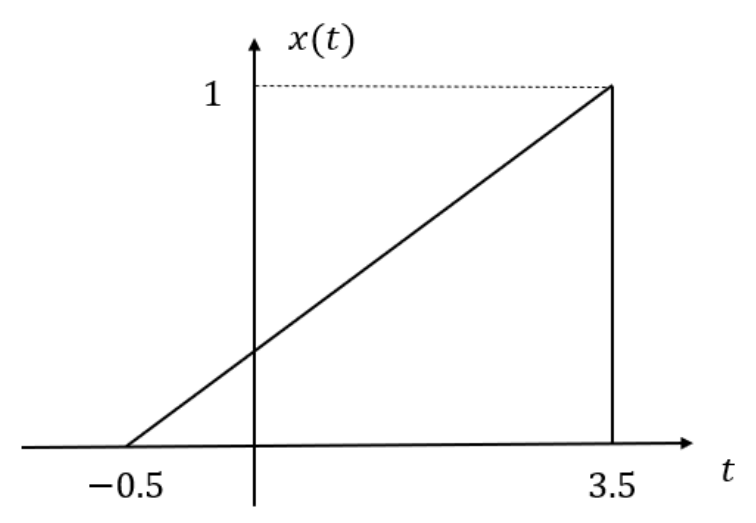
\includegraphics[width=0.5\textwidth]{img/figure1.png}
        \caption{Gráfica de la señal tipo "diente de sierra".}
        \label{figure1}
    \end{figure}

    En \cite{Sawtooth} se menciona que durante el intervalo en el que se presenta la señal, la función que 
    responde a una onda diente de sierra se da de la siguiente manera:
    
    \begin{equation*}
        x(t)=\frac{A}{T} t
    \end{equation*}

    Por lo que la función a la que responde la señal que se plantea debe ser del mismo modo, la expresión 
    de la señal es la siguiente:

    \begin{equation}
        x(t)=\frac{1}{4} t+\frac{1}{8}
        \label{equation3}
    \end{equation}

    Ahora que conocemos la expresión de la señal se procederá a obtener el valor del termino $a_{0}$, con las 
    ecuaciones \ref{equation2} y \ref{equation3}:

    \begin{equation*}
        a_{0}=\frac{1}{4} \int_{-\frac{1}{2}}^{\frac{7}{2}} \frac{1}{4} t+\frac{1}{8}
    \end{equation*}
    \begin{equation}
        a_{0}=\frac{1}{2}
        \label{equation4}
    \end{equation}    

    Para el valor de los términos restantes es importante mencionar que con frecuencia las simetrías simplifican 
    a los problemas matemáticos. En el caso de la series de Fourier, se utiliza la simetría en la paridad para 
    simplificar el problema. En el caso de funciones pares el desarrollo de la serie de Fourier implica solamente 
    la necesidad de calcular $a_{0}$ y $a_{n}$, y sólo $b_{n}$ para impares \cite{parimpar}.\\
    \\
    La señal que concierne a este texto podemos deducir de su gráfica(figura \ref{figure1}) que no se comporta igual que su imagen respecto 
    al eje $y$, ni tampoco hay presencia de simetría al rotar la gráfica en 180 grados. Por tanto, se trata de una 
    función sin paridad, lo que implica la necesidad de calcular todos los términos de la serie trigonométrica de Fourier .\\
    \\
    Las siguientes expresiones corresponden al calculo de los coeficientes $a_{n}$ y $b_{n}$:

    \begin{equation}
        a_{n}=\frac{2}{T} \int_{T} x(t)cos(2\pi nf_{0}t)dt
        \label{equation5}
    \end{equation}
    \begin{equation}
        b_{n}=\frac{2}{T} \int_{T} x(t)sin(2\pi nf_{0}t)dt
        \label{equation6}
    \end{equation}

    los resultados obtenidos al realizar los cálculos para los coeficientes son los siguientes (los cálculos que 
    se presentan en este documento están simplificados, por tal motivo se integra el paso a paso en el apartado de 
    Anexos):\\

    \begin{itemize}
        \item Calculo $a_{n}$
            \begin{equation*}
                a_{n}=\frac{1}{8}\int_{-\frac{1}{2}}^{\frac{7}{2}} tcos(2\pi nf_0t)dt + 
                \frac{1}{16} \int_{-\frac{1}{2}}^{\frac{7}{2}} cos(2\pi nf_0t)dt
            \end{equation*}
            \begin{equation}
                a_{n}=\frac{1}{\pi n} sin\left(\frac{7\pi n}{4}\right)+\frac{1}{2\pi^2 n^2}\left(cos\left(\frac{7\pi n}{4}\right)-cos\left(\frac{\pi n}{4}\right)\right)
                \label{equation7}
            \end{equation}
        \item Calculo $b_{n}$
            \begin{equation*}
                b_{n}=\frac{1}{8}\int_{-\frac{1}{2}}^{\frac{7}{2}} tsin(2\pi nf_0t)dt + 
                \frac{1}{16} \int_{-\frac{1}{2}}^{\frac{7}{2}} sin(2\pi nf_0t)dt
            \end{equation*}
            \begin{equation}
                b_{n}=-\frac{1}{\pi n} cos\left(\frac{7\pi n}{4}\right)+\frac{1}{2\pi^2 n^2}\left(sin\left(\frac{7\pi n}{4}\right)+sin\left(\frac{\pi n}{4}\right)\right)
                \label{equation8}
            \end{equation}
    \end{itemize}
    
    Lo siguiente sera completar la serie de Fourier para obtener la representación matemática de las funciones sinusoidales 
    que construyen la señal planteada, reemplazamos las ecuaciones \ref{equation7} y \ref{equation8} en la ecuación 
    \ref{equation1}:

    \begin{multline}
        x(t)=\frac{1}{2}+\sum_{n=1}^{\infty} \left[\frac{1}{\pi n} sin\left(\frac{7\pi n}{4}\right)+\frac{1}{2\pi^2 n^2}\left(cos\left(\frac{7\pi n}{4}\right)-cos\left(\frac{\pi n}{4}\right)\right)
        \right]cos\left(\frac{\pi nt}{2}\right)...\\ +\left[-\frac{1}{\pi n} cos\left(\frac{7\pi n}{4}\right)+\frac{1}{2\pi^2 n^2}\left(sin\left(\frac{7\pi n}{4}\right)+sin\left(\frac{\pi n}{4}\right)\right)
        \right]sin\left(\frac{\pi nt}{2}\right)
        \label{equation9}
    \end{multline}

    Ahora que se ha obtenido la expresión que representa la serie de Fourier de la señal, se procederá a realizar 
    un análisis de la serie de Fourier a través de una simulación realizada en computadora, en ella podremos 
    visualizar como se resuelve para cientos, o incluso miles, de componentes. Podemos comprobar qué tan buena 
    es la representación reconstruyendo la señal utilizando diferentes cantidades de componentes, para esto 
    se realizaran pruebas con un Script desarrollado en MATLAB.\\
    \\


    En esta sección explican de forma clara cómo fue el proceso para obtener los resultados:
    \begin{enumerate}
        \item Aspectos fundamentales de su simulación. No me refiero a pantallazos del código 
        (de hecho, eviten hacer eso en cualquier documento a menos de que les indiquen 
        lo contrario, en cuyo caso es más aconsejable mandarlo a un apéndice), sino a 
        consideraciones o suposiciones que hicieron para el planteamiento de la simulación, 
        con el fin de que ésta tenga congruencia con la teoría y por lo tanto validez. 

        \item Plan de pruebas. En caso de que su objetivo sea comprobar una hipótesis, entonces 
        deben plantear un plan de pruebas, es decir, mostrar la forma en la que proponen 
        variar parámetros de la simulación para crear diferentes escenarios que les permitan 
        hacer la validación. Busquen crear escenarios en los que varíen una cosa a la vez, 
        de tal forma que sea fácil interpretar los resultados, ya que saben qué es lo que está 
        influenciando los cambios. Si crean escenarios en los que todo cambia al mismo 
        tiempo, luego no será posible analizar el por qué de dichos resultados. 

        \item Para proyectos más grandes, como sus trabajos de grado, es necesaria una guía, 
        que permita plantear fases y conseguir una sumatoria resultados pequeños que 
        conduzcan al objetivo final, por eso en esos casos en esta sección se describe la 
        metodología utilizada; sin embargo, para nuestro caso no será así. 
    \end{enumerate}

\section*{Análisis de Resultados}
    Recuerden que presentar resultados no es lo mismo que adjuntar mil y una imágenes de 
    forma consecutiva. La sección de resultados es muy importante porque en ésta es en 
    donde ustedes realizan el análisis y ojo que ANÁLISIS ES DIFERENTE DE DESCRIPCIÓN.\\
    ... En la Figura 1 se observa que la línea roja por encima de la azul en todo 
    momento... (Muy amable por su descripción, pero eso también lo estoy viendo yo).\\
    ...Los resultados mostrados en la Figura 1 implican que para este escenario el método A 
    es superior al método B, debido a que con el método A se favorecen...\\
    La forma en la que ustedes interpretan lo que obtienen en la simulación me indica a mí su 
    dominio del tema. Si hay un resultado que no tiene sentido no traten de forzar sobre él 
    una explicación estrambótica, revisen si existen problemas en la simulación o el 
    planteamiento, pero para esto ustedes deben tener el tema claro, de lo contrario no 
    tendrán el criterio necesario para saber si el resultado tiene sentido o no.
    
\section*{Conclusiones}
    Aunque puede parecer que gastaron sus mejores ideas en la sección de análisis, la 
    diferencia de las conclusiones es que en este punto ustedes tienen una visión completa 
    del trabajo, ya han abordado todas las fases y por lo tanto están en la capacidad de 
    realizar un compendio de los aprendizajes obtenidos.\\
    Esos aprendizajes deben estar estrechamente relacionados con lo que buscan en el 
    trabajo, con lo que plantearon en el pro qué y el para qué en la introducción. Si esto fuera 
    su trabajo de grado, las conclusiones deben estar relacionadas con los objetivos de ese 
    trabajo.\\
    Lo anterior implica que la siguiente conclusión no es una conclusión válida:\\
    ... MATLAB es un entorno de simulación muy adecuado, ya que permite implementar 
    sistemas de telecomunicaciones...

\begin{thebibliography}{99}
    \bibitem{diapositivas}
        M. Silva, “Capítulo II: Análisis de Fourier,” Notas Cl., pp. 3–70, 2021.
    \bibitem{Sawtooth}
        A. Engineering, M. Subject, L. Transform, and O. F. Periodic, “Snpit \& rc,” p. 11, [Online]. Available: https://www.slideshare.net/surtikaushal/laplace-periodic-function-with-graph.
    \bibitem{parimpar}
        E. Rojero, “Matemáticas Avanzadas,” Univ. Nac. Autónoma México, vol. 0.1, p. 52, 2009, [Online]. Available: https://openlibra.com/es/book/download/matematicas-avanzadas.
\end{thebibliography}
\end{document}
